\section{State of the art in ESD testing}

To ensure proper operation once in the field, hardware is tested against ESD using different test methods and standards.
The goal for each method is to reproduce a particular ESD waveform in lab conditions.
In this chapter, we will introduce most relevant ESD generators, which will be useful later on for modeling them accurately.

\subsection{Transmission Line Pulsing (TLP)}
Transmission Line Pulsing uses the discharge of a cable to generate a fast and square pulse.
It is extensively used in the ESD field \cite{TLP, TLPforESDProtectionCz, TLPthroubleshooting, LacrampeTransientImmunity}, for characterization purpose or day-to-day testing of devices.

\subsection{ESD Gun (IEC 61000-4-2 / ISO 10605)}
blabla

\subsection{ISO 7637-2}

\subsection{Burst test (IEC 61000-4-4)}

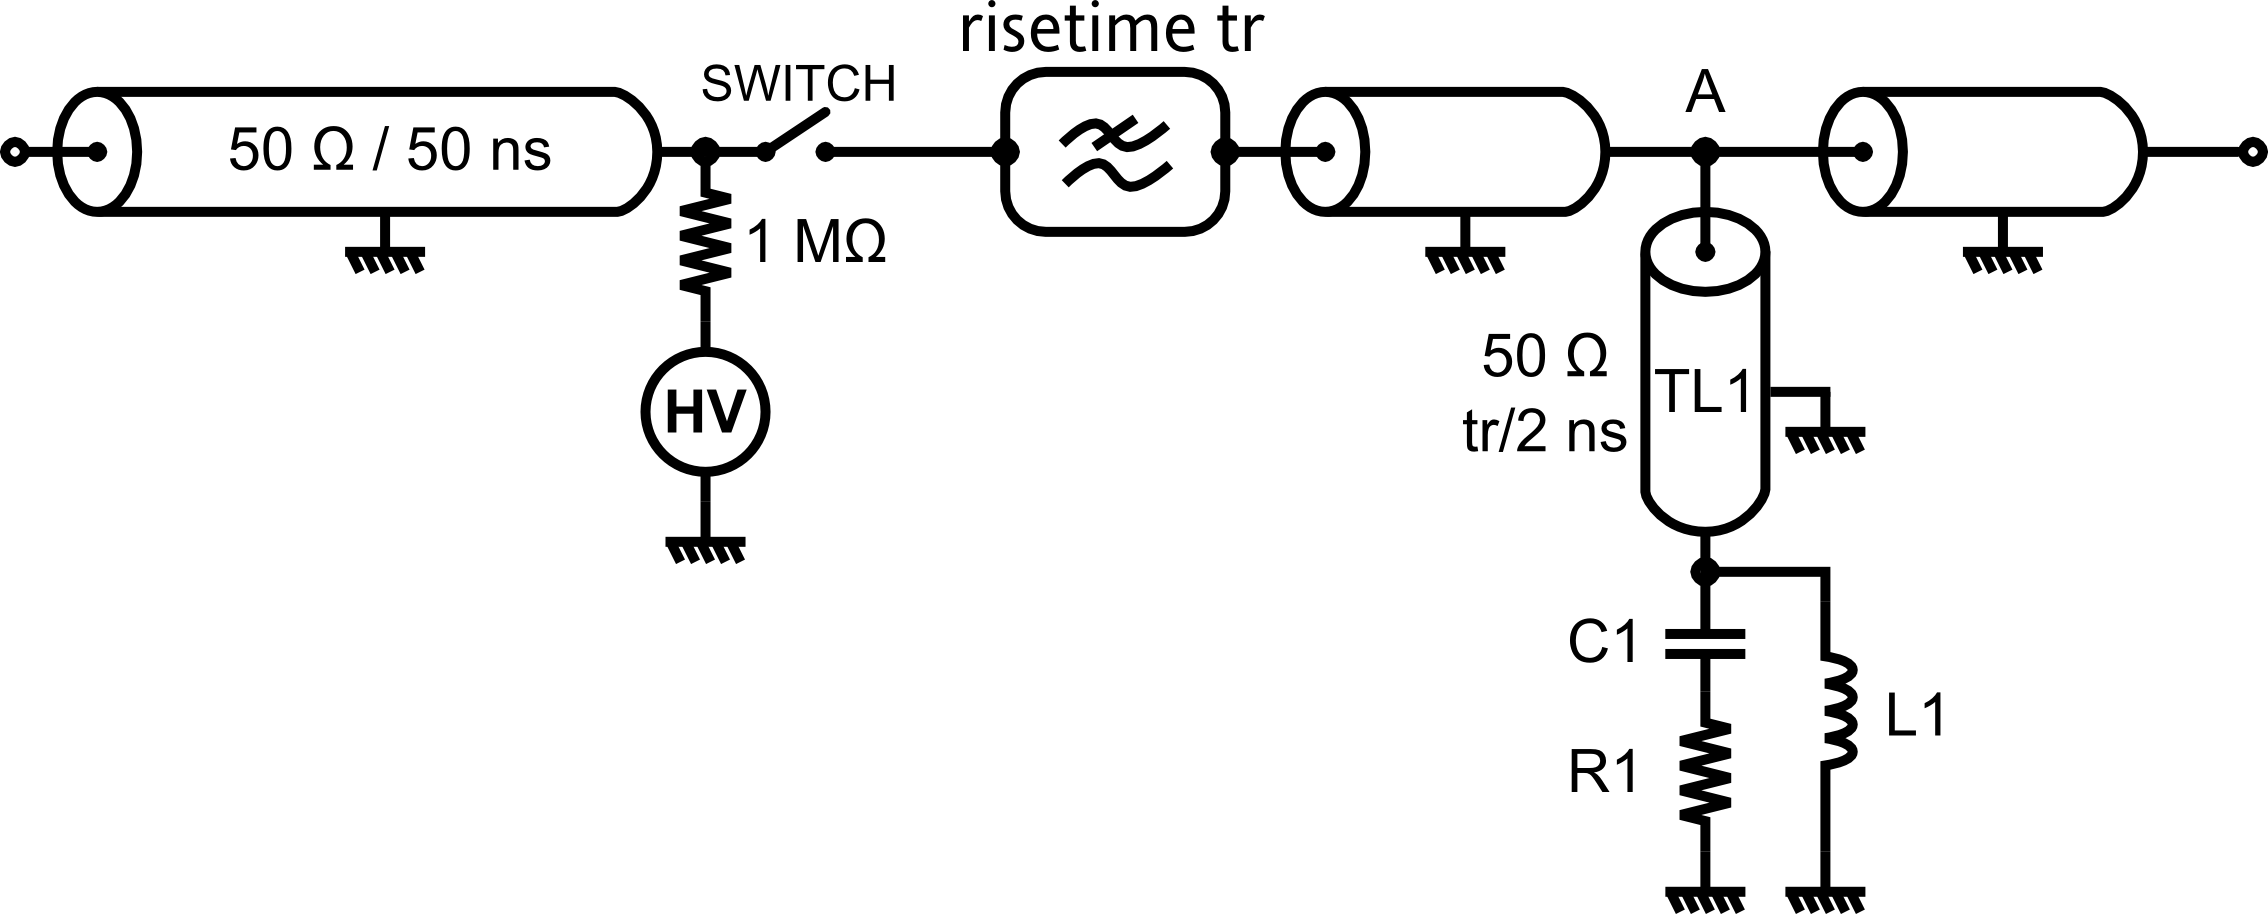
\includegraphics[width=\textwidth,height=\textheight,keepaspectratio]{src/2/figures/tlp_iec.png}
